
\section{Unified Modeling Language (UML)}
\label{sc:UML}
\subsection{Historie und Ziel}
Die \acs{UML} ist eine durchgängige Modellierungssprache von der
organisatorischen Beschreibung von Geschäftsprozessen bis zu direkt ausführbaren Modellen,
d.h. bis zur Implementierung. Sie ist über ISO standardisiert (ISO /IC 19501).\\
Ein erster Ansatz wurde 1990 auf der Grundlage verschiedener Notationssysteme entwickelt.
Die Standardisierung, Pflege und Weiterentwicklung der Sprache wurde an die OMG
übergeben, die die Sprache im Jahr 1997 zur Version \ac{UML} 1.1 weiterentwickelte. Seit Ende der
1990er Jahre haben zahlreiche Personen und Institutionen intensiv an der \ac{UML} Version 2.0
gearbeitet, die im Jahr 2006 vollständig fertig gestellt und Anfang 2009 von der leicht
überarbeiteten Version 2.2 abgelöst wurde. Eine Standardisierung durch die International
Standardization Organization (ISO) hat die Version 2.2 allerdings noch nicht erreicht. Diese bleibt bisher nur der Version 1.4.2 vorbehalten \cite{MT001}.
\subsection{Metamodell} 
UML legt Spracheinheiten fest, die auf verschiedenen Ebenen agieren. Mit diesen drücken sie die Struktur und das Verhalten eines Systems aus. Einige Elemente nutzt die Modellierungssprache, um sich selbst zu definieren \cite{MT001}. Die Meta-Modellierung umfasst alle Elemente von \ac{UML}, auch solche, die \ac{UML} selbst beschreiben. Dafür nutzt es vier hierarchisch angeordnete Ebenen (M0 bis M3).

Die Meta-Metaebene M3 spezifiziert die Metadaten der Modellierungssprache und deren Zusammenhänge mithilfe der Meta Object Facility (MOF). Sie definiert das Metamodell. Zudem befähigt Sie den Metadaten-Transfer. Das von der OMG definierte Format XMI ist ein praktisches Tool, um objektorientierte Daten auf Meta-Metaebene zwischen Entwicklungstools zu teilen. Die Object Constraint Language (OCL), eine deklarative Programmiersprache, ergänzt \ac{UML} und reguliert Randbedingungen der jeweiligen Modellierung. Als Textsprache wirkt sie jedoch nur unterstützend, statt selbst für Modellierung zur Verfügung zu stehen.

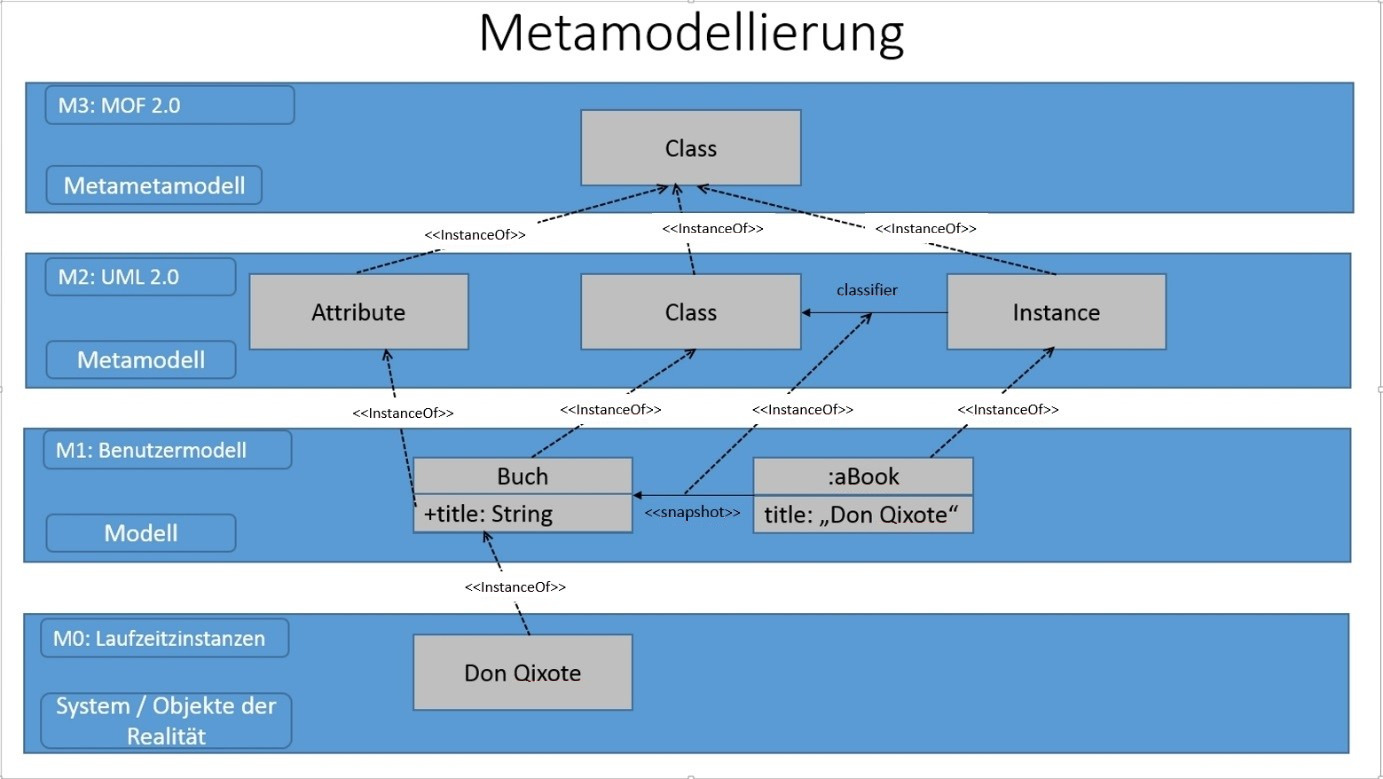
\includegraphics[scale=0.7]{Graphics/metamodell}
\captionof{figure}{Die Metamodellierung zeigt die hierarchische Beziehung zwischen den Sprachebenen}
\label{fig1}


Die obere Grafik zeigt die Metamodellierung von UML 2.0. Ebene M0 ist die grundlegende Ebene. Sie stellt konkrete, reale Objekte und einzelne Datensätze dar – z. B. ein Objekt oder eine Komponente. Ebene M1 umfasst alle Modelle, die die Daten der Ebene M0 beschreiben und strukturieren \cite{MT009}. Das sind UML-Diagramme wie das Aktivitätsdiagramm oder das Paketdiagramm (weiter unten erklärt). Um den Aufbau dieser Modelle zu definieren, legen Metamodelle der Ebene M2 die Spezifikationen und Semantik der Modellelemente fest.\\

Wollen Sie ein verständliches UML-Diagramm erstellen, müssen Sie das Metamodell UML mit seinen Regeln kennen. Die höchste Ebene, M3, ist ein Metamodell des Metamodells. Die erwähnte Meta Object Facility arbeitet auf einer abstrakten Ebene, die Metamodelle definiert. Diese Ebene definiert sich selbst, da sonst weitere, übergeordnete Meta-Ebenen entstünden.\\

\subsection{Kurzbeschreibung}
Bei der Unified Modeling Language (UML) handelt es sich nicht um eine bestimmte Methode, sondern vielmehr um einen Sammelbegriff für grafische Methoden der objektorientierten Entwicklung und Dokumentation von Software (Object Oriented Design – OOD). Dies umfasst Methoden und Notationen für Planung, Design, Entwurf und Implementierung von Software, die seit den 90er Jahren durch die Object Management Group (die auch BPMN pflegt) zu einem offiziellen Standard, der UML, zusammengeführt wurden.\cite{MT005} \\
Im Gegensatz zu anderen Methoden, die primär auf die Modellierung von Prozessen abzielen, kann die UML direkt zur Software-Entwicklung genutzt werden.\\
Die objektorientierte Sichtweise, auf der UML basiert, zieht ausgehend von der realen Welt Objekte heraus, die mit Attributen beschrieben werden. Die Objekte werden zu Klassen verdichtet, wenn Eigenschaften und Verhalten der Objekte identisch oder ähnlich sind. Klassen können daher als Baupläne für die zu erzeugenden Objekte (die Instanzen einer Klasse) interpretiert werden. Die Objekte, Klassen, Attribute und Methoden bilden die Basis für sämtliche Diagrammtypen der UML. Die verschiedenen Diagrammtypen können in\\

 statische Modelle (-> Strukturdiagramme)\\
• das Klassendiagramm,\\
• das Kompositionsstrukturdiagramm (auch: Montagediagramm),\\
• das Komponentendiagramm,\\
• das Verteilungsdiagramm,\\
• das Objektdiagramm,\\
• das Paketdiagramm und\\
• das Profildiagramm.\\
und\\
 dynamische Modelle (-> Verhaltensdiagramme)\\
• das Aktivitätsdiagramm,\\
• das Anwendungsfalldiagramm (auch: Use-Case o. Nutzfalldiagramm),\\
• das Interaktionsübersichtsdiagramm,\\
• das Kommunikationsdiagramm,\\
• das Sequenzdiagramm,\\
• das Zeitverlaufsdiagramm und\\
• das Zustandsdiagramm\\
unterteilt werden.\\
Statische Modelle (wie z.B. das Klassendiagramm) zeigen die Beziehungen zwischen den Klassen und den beteiligten Akteuren auf. Demgegenüber zeigen dynamische Modelle (wie z.B. das Sequenzdiagramm) den Prozessablauf auf. Aufgrund der Vielzahl an Diagrammtypen ergeben sich vielfältige Anwendungsmöglichkeiten, da jeder Typ eine spezifische Sicht auf den zu modellierenden Prozess sowie das System ermöglicht\cite{MT009}.\\
Im Folgenden werden einige ausgewählte UML-Diagrammtypen erläutert, wobei jeweils der Nutzen im Rahmen des Geschäftsprozessmanagements herausgearbeitet wird.\\
\\
\\
\\
Das Anwendungsfalldiagramm (use case diagram) dient im Rahmen der Softwareentwicklung dem Einstieg in die Anforderungsanalyse. Gleichzeitig kann es zur Darstellung der relevanten Geschäftsprozesse einschließlich der Beziehung zu den an den Prozessen beteiligten Personen genutzt werden. Ein Anwendungsfall entspricht hierbei entweder einem Geschäftsprozess oder einem Teilprozess. Durch das Anwendungsfalldiagramm kann dann dargestellt werden, welche Akteure an den betrachteten Prozessen beteiligt sind und welche Prozesse weitere Prozesse beinhalten. Die Akteure sind dabei im Sinne von Rollen eines Benutzers innerhalb des Systems zu verstehen, wobei diese nicht zwingend menschlich sein müssen. Dies ist beispielsweise der Fall, wenn ein anderes System eingebunden wird. Die Anwendungsfälle werden in diesem Diagrammtyp über Ellipsen abgebildet, während die Akteure als Strichmännchen dargestellt werden. Die Beziehungen zwischen dem Anwendungsfall und den beteiligten Akteur werden über ungerichtete Kanten visualisiert.\\



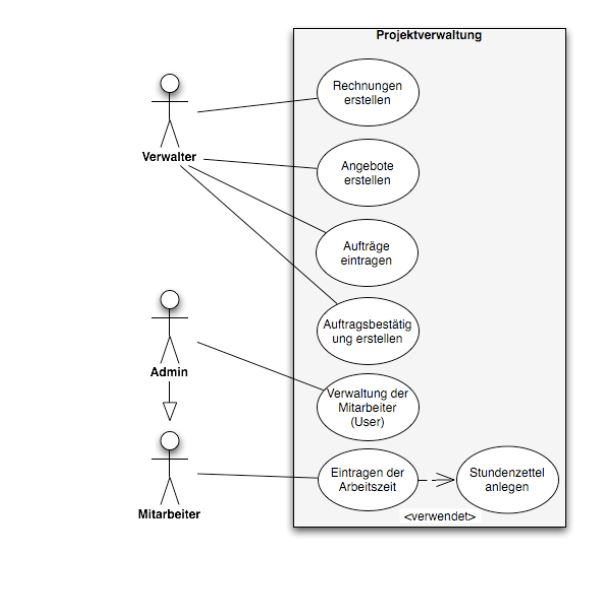
\includegraphics[scale=0.8]{Graphics/Anwendungsdiagram.jpg} 
\captionof{figure}{Beispiel eines Anwendungsfalldiagramms in UML}
Quelle : \cite{MT005}


Anwendungsfalldiagramme weisen jedoch den Nachteil auf, dass keine Reihenfolge bei der Bearbeitung der Anwendungsfälle abgebildet werden kann. Es wird somit nicht deutlich, welcher Anwendungsfall vor einem anderen durchgeführt werden muss. Allerdings kann diese Reihenfolge beispielsweise durch andere Methoden der UML, wie das Aktivitätsdiagramm, kompensiert werden. Zudem muss jeder Anwendungsfall anhand einer Beschreibung dokumentiert werden. Hierbei bestehen jedoch keine Vorgaben, weshalb sich Inkonsistenzen und Redundanzen ergeben können. Darüber hinaus kann nicht sichergestellt werden, dass Dritte die Dokumentation auch verstehen. Daher sollte auf Vorlagen, die nicht offiziell zum Standard der UML gehören, zurückgegriffen werden.\cite{MT005} \\


Das Klassendiagramm (Class Diagram) eignet sich zur Darstellung von Klassenstrukturen innerhalb eines IKS. Klassendiagramme können nicht direkt für die Geschäftsprozessmodellierung verwendet werden. Stattdessen handelt es sich eine statische Darstellung von Klassen, Objekten und deren Beziehungen untereinander. Klassendiagramme beschreiben jedoch nur, dass eine Interaktion besteht; wie diese ausgestaltet ist kann jedoch nicht dargestellt werden.\\


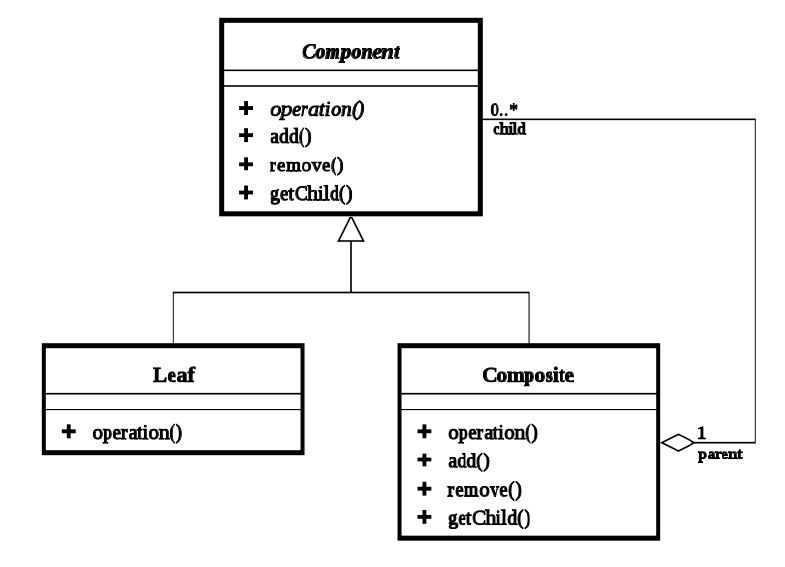
\includegraphics[scale=0.7]{Graphics/Klassendiagram.jpg} 
\captionof{figure}{Beispiel eines Klassendiagramms in UML}



Quelle : \cite{MT005}


Das Aktivitätsdiagramm oder auch Ablaufdiagramm (Activity Diagram) wird zur Darstellung von Abläufen verwendet. Im Mittelpunkt steht dabei die Visualisierung paralleler Abläufe\cite{MT005}. Aus diesem Grund eignet sich dieser Diagrammtyp in einem besonders hohen Maße zur Abbildung von Geschäftsprozessen, da diese zumeist Parallelitäten vorweisen. Aktivitätsdiagramme sind darüber hinaus zur Modellierung von Workflows und zur Verfeinerung von Anwendungsfällen geeignet. Des Weiteren sind Aktivitätsdiagramme in der Lage unterschiedliche Detaillierungsgrade wiederzugeben. So ist es unter anderem möglich ein anwendungsfallübergreifendes Diagramm zu erzeugen und anschließend die darin enthaltenen Anwendungen einzeln zu modellieren.\\

   

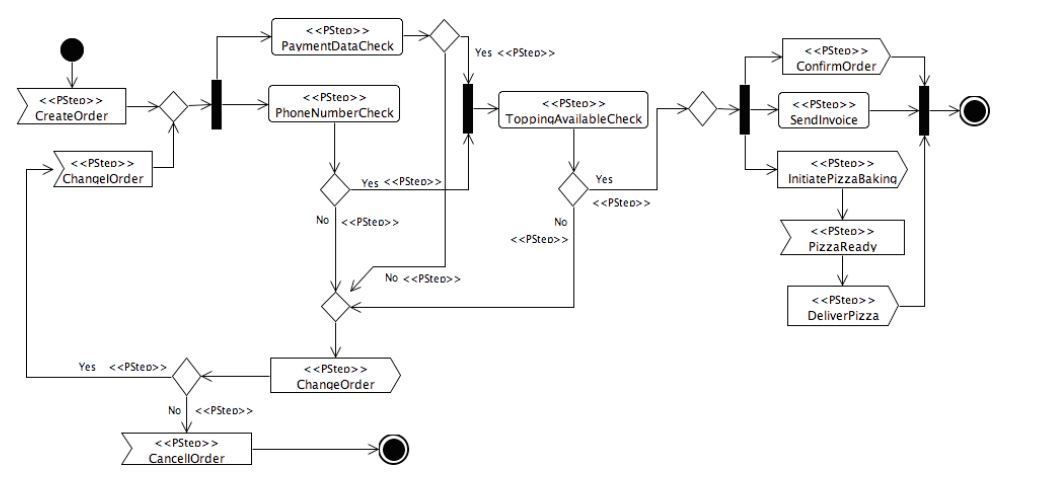
\includegraphics[scale= 0.65]{Graphics/activitydiagram.jpg} 
\captionof{figure}{Beispiel eines Aktivitätsdiagramm in UML}



Quelle : \cite{MT005}


\subsection{UML-Diagramme: Eine Übersicht}
Die folgende Übersicht zeigt übergeordnete Kategorien und Anwendungsmöglichkeiten der einzelnen Diagrammtypen in Kurzform. Wenn Sie ein modellorientiertes Software-System, einen Anwendungsfall in der Wirtschaft o. Ä. visuell darstellen wollen, sollten Sie laut Empfehlung der UML-Task-Force vorher einen der UML-Diagrammtypen wählen. Erst dann lohnt es sich, eines der vielen UML-Tools zu wählen, da diese häufig eine gewisse Methode vorschreiben. Dann erstellen Sie das UML-Diagramm.\cite{MT011} \\

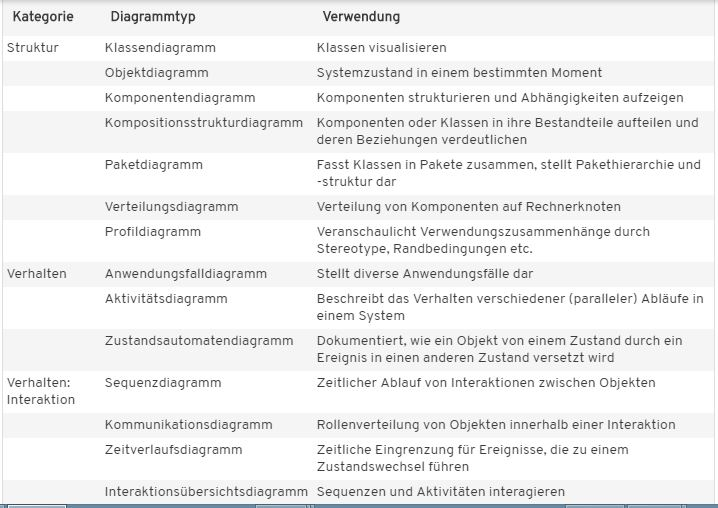
\includegraphics[scale=1]{Graphics/UMLdiagramme.jpg} 
\captionof{figure}{UML-Diagramme}


 

\subsection{Vor- und Nachteile im Überblick}
UML ist heute eine der dominierenden Sprachen für die Modellierung von betrieblichen Anwendungs- bzw. Softwaresystemen. Der erste Kontakt zu UML besteht häufig darin, dass UML-Diagramme im Rahmen von Softwareprojekten zu erstellen, zu verstehen oder zu beurteilen sind\cite{MT005}. UML-Diagramme gelten als Standard bei objektorientierter Modellierung.\\

   

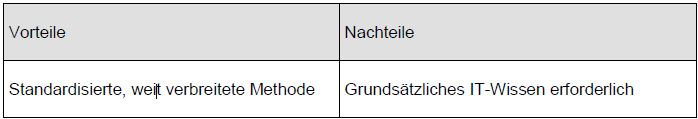
\includegraphics[scale=0.9]{Graphics/vornach.jpg}
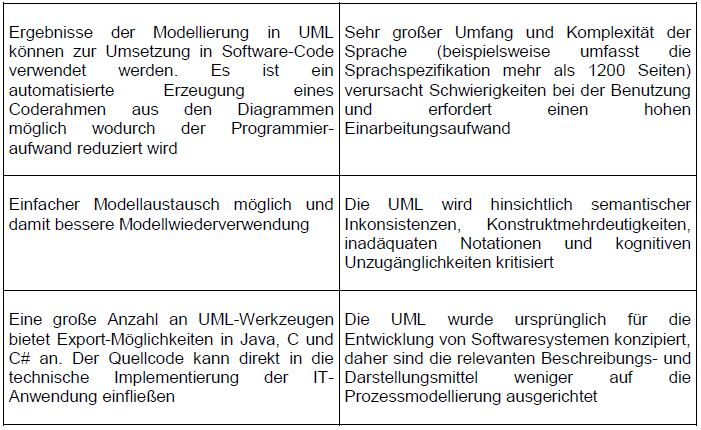
\includegraphics[scale=0.9]{Graphics/vornach2.jpg} 
\captionof{figure}{UML: Vor- und Nachteile }


Quelle : \cite{MT005} 

 
